\chapter{新玩具}

\begin{quote}
    我属我的良人,他也恋慕我。我的良人,来吧,你我可以往田间去。你我可以在村庄住宿!我们早晨起来往葡萄园去,看看葡萄发芽开花没有,石榴放蕊没有。我在那里要将我的爱情给你。

    \hfill《圣经·雅歌》7:11
\end{quote}

在本章,我会介绍专为本书创建的工具。为了看懂本章定义的大部分指令和环境,你需要阅读过第9章和第10章的内容……本章中,我们会涉及带有“危险”标记的提示的创建方法、各章开头的首字下沉、摘要、术语字典、带有当前章号的标签,以及并列展示\LaTeX 代码和效果的环境。

\section{一些小手工}

\subsection{参数和排版转换}

在涉及信息语言的文档中,需要突出显示参数、指令,以及函数。例如,我们需要这类效果:

\begin{codelist}[11.1]{
    为了编译文件\codereplace{文件}:
\begin{flushleft}
    \ttfamily latex \codereplace{文件}
\end{flushleft}
}
\begin{verbatim}
为了编译文件\bwarg{文件}:
\begin{flushleft}
    \ttfamily latex \bwarg{文件}
\end{flushleft}\end{verbatim}
\end{codelist}

指令\verb|\bwmarg|可以以\textsl{倾斜字体}来输出其参数,并且置于“⟨”和“⟩”之间。这种括号可以在数学模式下分别由指令\verb|\langle|、\verb|\rangle|生成。此外,你无疑注意到了,我们可以使用下标符号,就像这样:

\begin{codelist}[11.2]{
复制文件:
\begin{flushleft}\ttfamily
    cp \codereplace{文件$_1$} ...
    \codereplace{文件$_n$}
    \codereplace{文件$_{dst}$}
\end{flushleft} 
}
\begin{verbatim}
复制文件:
\begin{flushleft}\ttfamily
    cp \bwarg[1]{文件} ...
    \bwarg[n]{文件}
    \bwarg[dst]{文件}
\end{flushleft}\end{verbatim}
\end{codelist}

指令\verb|\bwarg|\jz{
    这个名称代表“黑白”参数(« black \& white » argument)……
}的定义如下:

\begin{dmd}
\begin{verbatim}
\newcommand{\marg}[2][]{% 
    {\normalfont%
        \textsl{$\langle$#2%
            % 如果选用了可选参数 
            \ifthenelse{\equal{#1}{}}{} 
            {$_\mathit{#1}$}% 显示下标
            $\rangle$}}}%\end{verbatim}
\end{dmd}

指令\verb|\normalfont|的效果是回到文档的默认字体。这解释了为什么示例11.1中的“\codereplace{文件}”没有使用打字机字体显示。

在本文档的电子版(也就是需要通过屏幕阅读的版本)中,我们决定使用\emph{颜色}而不是字符“⟨”和“⟩”。这样一来,可以定义指令\verb|\colarg|:

\begin{dmd}
\begin{verbatim}
\newcommand{\colarg}[2][]{{% 
    \normalfont\color{blue!90}#2% 蓝色 
    \ifthenelse{\equal{#1}{}}{}{$_\mathit{#1}$}}}\end{verbatim}
\end{dmd}

接下来,借助一个巧妙放置的布尔值\celan{\S 9.3.1},我们可以定义一个通用的指令\verb|\marg|,以调用其中的一个版本(黑白版本或彩色版本):

\begin{dmd}
\begin{verbatim}
\ifversionenligne
    \let\marg\colarg
\else
    \let\marg\bwarg
\fi\end{verbatim}
\end{dmd}

这个结构调用了\TeX 的指令\verb|\let|,在9.2.3小节有明确的介绍。

\subsection{关于索引的生成}

本书中,凡是行文中提到指令、环境、包、文档类型等时,都会调用对应的特殊指令,来自动在索引中插入一条入口\yz{
    妈的怎么不早说。算了先不做索引了,全书翻译完之后再调整吧。
}。举例来说,这样一来的效果为:

\begin{codelist}[11.3]{
借助包\textsf{varioref},可以
使用指令\dm{\backslash vref}……
}
\begin{verbatim}
借助包\ltxpack{varioref},可以
使用指令\ltxcom{vref}……\end{verbatim}
\end{codelist}

指令\verb|\ltxpack|的定义如下。首先,以下内容定义的指令\verb|\ltx@pack|可以以非衬线字体展示包名:

\begin{dmd}
\begin{verbatim}
\newcommand{\ltx@pack}[1]{%
    \upshape\textsf{#1}}\end{verbatim}
\end{dmd}

接下来,我们像这样定义:

\begin{dmd}
\begin{verbatim}
\newcommand{\ltxpack}[1]{%
    \ltx@pack{#1}% 
    \protect\index{扩展们!\protect\texttt{#1}}% 
    \protect\index{#1@\protect\textsf{#1 扩展}}}\end{verbatim}
\end{dmd}

其中调用了前面定义的指令,并在索引中插入了两个入口,一个遵循“\codereplace{包名}扩展”的格式,另一个作为“扩展们”的\celan{\S 6.3}子入口。这里,指令\verb|\protect|的作用是避免指令\verb|\ltxpack|本身作为作为另一条指令的参数时带来的麻烦。遵循同样的思路,我们可以定义指令\verb|\ltxcom|。首先:

\begin{dmd}
\begin{verbatim}
\newcommand{\ltx@com}[1]{%
    \texttt{\symbol{92}#1}}\end{verbatim}
\end{dmd}

以上指令可以以打字机字体生成指令名,并在前面加上字符\dm{\backslash}。\verb|\symbol|是\LaTeX 指令,此处用于插入所选字体下的第92个字符(恰好为反斜杠)。因此,我们最终有如下定义:

\begin{dmd}
\begin{verbatim}
\newcommand{\ltxcom}[1]{%
    \ltx@com{#1}% 
    \index{#1@\protect\texttt{\symbol{92}#1}}}\end{verbatim}
\end{dmd}

该指令调用了上一条指令,在索引中插入一个入口。此处需要提炼出的思想是,定义可以自动在索引中插入入口的指令可能很有帮助。举例来说,我们也许可以定义这样一条指令:

\begin{dmd}
\begin{verbatim}
\newcommand{\jargonanglais}[1]{% 
    \emph{#1}%
    \index{#1}}\end{verbatim}
\end{dmd}

该指令可以在设置英文术语格式的同时将其插入索引——比如某个特殊的索引。同样,如果在文档中经常出现,我们就可以定义一条指令,将其插到索引中。例如,在本书中,我们有这样的定义:

\begin{dmd}
\begin{verbatim}
\newcommand{\postscript}{% 
    PostScript% 
    \protect\index{PostScript}}\end{verbatim}
\end{dmd}

\subsection{跳转提示}

本书的纸质版中四处分散着跳转阅读的提示,例如这个提醒你去看\celan{\S D.3.5}术语字典(glossaire)的提示——幸亏我们这里在说跳转阅读,否则这个术语字典就这里的内容毫无关联了\jz{
    如果你没完全跟上的话,我是想说,这里其实没有术语字典的什么事……
}。实现跳转提示符号的指令被赐名为\verb|\voir|,接收两个参数:

\begin{dmd}
\backslash voir\{\codereplace{目标标签}\}\{\codereplace{跳转对象文本}\}
\end{dmd}

例如,前面的跳转是这样生成的:

\begin{dmd}
\verb|\voir{chap-glossaire}{glossaire}|
\end{dmd}

这个指令的设计过程中,全部的“难点”在于怎样让三角形根据页面奇偶性来改变朝向。借助包\textsf{chngpage},这一难点得以功课。请参阅9.3.3小节。

余下的工作就是展示三角形。为了达成这一目的,我们定义了两个指令,分别生成侧栏的跳转提示和正文中的标记。由此,\verb|\voir|的格式如下:

\begin{dmd}
\begin{verbatim}
\newcommand{\voir}[3][\S]{% 
    \checkoddpage% 
    \ifcpoddpage
        \v@irpageimpaire{#1}{#2}{#3}}{% 奇数页的跳转提示
    \else
        \v@irpagepaire{#1}{#2}{#3}}} % 偶数页的跳转提示
    \fi\end{verbatim}
\end{dmd}%TODO 此处括号似乎不配对

我们注意到,除了两个必需的参数外,该指令还可以接收一个可选参数,它默认定义为段落标记(\S)。指令\verb|\v@irpageimpaire|和\verb|\v@irpagepaire|是对称的,作用如下:

\begin{enumerate}
    \item 将“朝向正确”的三角形放置在文本中,作为跳转提示对象;
    \item 在侧栏生成带有跳转目标的注解。
\end{enumerate}

三角形可以从包\textsf{amssymb}中包含的符号中获取:

\begin{codelist}[11.4]{
    天啊,那些“美观”的三角形:
$\blacktriangleleft$和
$\blacktriangleright$!
}
\begin{verbatim}
天啊,那些“蟀爆了”的三角形:
$\blacktriangleleft$和
$\blacktriangleright$!\end{verbatim}
\end{codelist}

如下所示,是针对在偶数页实现跳转提示的指令的最终版本:

\begin{dmd}
\begin{verbatim}
\newcommand{\v@irpageimpaire}[3]{% 
    {\tiny$\blacktriangleright$}#3% 文本中的跳转提示
    \marginpar{%
        \parbox[t]{.9\marginparwidth}{% 
            {\footnotesize\sffamily%
                \hfill#1~\ref{#2}}~{\small$\blacktriangleleft$}\\
            {\footnotesize\sffamily%
                \mbox{}\hfill p.~\pageref{#2}\hfill\mbox{}}}}\end{verbatim}
\end{dmd}% TODO 括号配对

注意到,在侧栏的跳转内容包含于一个\verb|\parbox|\celan{\S 4.4.3},其中分两行展示章节编号和页码\yz{
    中文版暂时没做页码。%TODO 页码
}。对于奇数页,需要做与偶数页相同的事情,只不过需要考虑到它是奇数页\dm{:-)}

在“在线”版本中,跳转提示可以像超文本链接(lien hypertexte)那样呈现。这可以简单地通过指令\verb|\hyperref|(对应包同名)来实现。因此,我们可以编写出这类指令:

\begin{dmd}
\begin{verbatim}
\newcommand{\voir}[3][\S]{% 
    \hyperref[#2]{#3}}\end{verbatim}
\end{dmd}

其中的可选参数没有过多的用处,只是为了与“纸质”版本中的指令\verb+\voir+兼容。

\subsection{更改侧栏}

在本文中,我多次临时改变了侧栏的样子,尤其是针对用于并列展示\LaTeX 代码和其效果,或需要展示题记等内容%TODO 是题记吗?
的情况。为了实现这种效果,维护\LaTeX 法文问答社区的玛丽-保罗·克卢特(Marie-Paul Kluth)\jz{
    这位似乎有个命中注定的姓[lom prédestilé;译注:将nom prédestiné中的n替换为了l。此处是在调侃此人的姓(Kluth)与发明\TeX 的克努特(Knuth)仅有一个字母的区别]……
}提议使用一种集成环境,如下所示:

\begin{dmd}
\begin{verbatim}
\newenvironment{changemargin}[2]% 
    {\begin{list}{}{%
        \setlength{\listparindent}{\parindent}% 
        \setlength{\itemindent}{\parindent}% 
        \setlength{\leftmargin}{#1}% 
        \setlength{\rightmargin}{#2}%
    }\item }% 
    {\end{list}}\end{verbatim}
\end{dmd}

其中的思路是定义一个列表,而我们修改其中的侧栏。该环境接收的两个参数分别代表左侧和右侧的边距尺寸。这样的思路可以让环境产生很有趣的结果:边距会根据页面的奇偶性而实用不同的尺寸。这样的环境可以定义如下:

\begin{dmd}
\begin{verbatim}
\newenvironment{agrandirmarges}[2]{% 
    \begin{list}{}{%
        \setlength{\topsep}{0pt}% 
        \setlength{\listparindent}{\parindent}% 
        \setlength{\itemindent}{\parindent}% 
        \setlength{\parsep}{0pt plus 1pt}% 
        \checkoddpage%
        \ifcpoddpage
            \setlength{\leftmargin}{-#1}
            \setlength{\rightmargin}{-#2}
        \else
            \setlength{\leftmargin}{-#2}
            \setlength{\rightmargin}{-#1}
        \fi}\item }% 
    {\end{list}}\end{verbatim}
\end{dmd}

\newenvironment{agrandirmarges}[2]{% 
    \begin{list}{}{%
        \setlength{\topsep}{0pt}% 
        \setlength{\listparindent}{\parindent}% 
        \setlength{\itemindent}{\parindent}% 
        \setlength{\parsep}{0pt plus 1pt}% 
        \checkoddpage%
        \ifcpoddpage
            \setlength{\leftmargin}{-#1}
            \setlength{\rightmargin}{-#2}
        \else
            \setlength{\leftmargin}{-#2}
            \setlength{\rightmargin}{-#1}
        \fi}\item }% 
    {\end{list}}

注意,这里我们使用了指令\verb|\isodd|来测试页面的奇偶性。图\ref{fig:11.1}展示了使用这种环境的示例,其代码如下:

\begin{figure}[bt]
    \centering
    \newcommand{\graphtex}{%
      
\includegraphics[height=2cm]{img/knuth-tex}}
    \begin{agrandirmarges}{1cm}{2cm}
      \begin{center}
        \graphtex\graphtex\graphtex\graphtex\graphtex%
        \graphtex\graphtex\graphtex\graphtex\graphtex%
        \graphtex\graphtex\graphtex\graphtex\graphtex%
        \graphtex\graphtex\graphtex\graphtex%
      \end{center}
    \caption{一幅内容完全不重要的图。它的出现只是为了说明我们可以在需要额外空间的时候临时修改左边距和右边距……}
    \label{fig:11.1}
    \end{agrandirmarges}
\end{figure}

\begin{dmd}
\begin{verbatim}
    \begin{figure}[tb]
        \begin{agrandirmarges}{1cm}{2cm}
            % 这里1cm针对“订口”侧
            %     2cm针对“切口”侧
        ...
        \caption{一幅内容完全不重要的……}
        \end{agrandirmarges}
      \end{figure}\end{verbatim}
\end{dmd}

\section{各种提示}

提示中可以见到的符号来源于“剪贴画”(……)。在图\ref{fig:11.2}中以3 cm的宽度展示了这些符号。在文档对应位置插入这些符号的“提示”由鄙人定义的环境生成。环境基于\TeX 层面的一项功能,而这项功能正是我勤勉地阅读\TeX Book是发现的,那就是指令\verb|\parshape|。该指令可以为段落指定任意形状:

\begin{codelist}[11.5]{
\parshape=5
1.5cm 2.5cm
1.5cm 2.5cm
1cm 2cm
1cm 2cm
0pt \textwidth 
a a a a a a a a a a a a a a a a a a a 
a a a a a a a a a a a a a a a a a a a 
a a a a a a a a a a a a a a a a a a a 
}
\begin{verbatim}
\parshape=5
1.5cm 2.5cm
1.5cm 2.5cm
1cm 2cm
1cm 2cm
0pt \textwidth 
a a a a a a a a a a a a a a a a a a a 
a a a a a a a a a a a a a a a a a a a 
a a a a a a a a a a a a a a a a a a a \end{verbatim}
\end{codelist}

\begin{figure}[htb]
    \begin{center}
      
\includegraphics[width=3cm]{img/fmb-important}\quad%
      
\includegraphics[width=3cm]{img/fmb-note}\quad%
      
\includegraphics[width=3cm]{img/fmb-question}
    \end{center}
    \caption{手册中使用的符号}
    \label{fig:11.2}
\end{figure}

符号“=”后面的数字用于指明我们想要变形的行数。接下来,成对出现的数字用于指明缩进和该行变形后的长度。对于上述示例,有:

\begin{itemize}
    \item 最先出现的两行缩进1.5 cm,并且每行长2.5 cm;
    \item 接下来的两行缩进1 cm,并且每行长2 cm;
    \item 第五行(也是最后一次指明内容)可以决定接下来所有行的风格,即缩进0 cm且行长等于事先定义的长度\verb|\textwidth|。
\end{itemize}

因此,想要在段落中插入提示,我们可以借助该指令将前两行错位:

% \newlength{\larnota}
% \newlength{\largligne}

\begin{codelist}[11.6]{
\setlength{\larnota}{.9cm}
\setlength{\largligne}{%
    \textwidth-\larnota}
\parshape=3
\larnota\largligne
\larnota\largligne
0pt\textwidth
\noindent 注意,这个段落唯一的
作用,就是用来证明我们确实可以
将段落中的两行内容错后一些,并
让随后的内容如同什么都没有发生
一样继续……
}
\begin{verbatim}
\setlength{\larnota}{.9cm}
\setlength{\largligne}{%
    \textwidth-\larnota}
\parshape=3
\larnota\largligne
\larnota\largligne
0pt\textwidth
\noindent 注意,这个段落唯一的
作用,就是用来证明我们确实可以
将段落中的两行内容错后一些,并
让随后的内容如同什么都没有发生
一样继续……\end{verbatim}
\end{codelist}

好了,接下来要做的事情就是在指令\verb|\parshape|留下的“洞口”中放上图片,让我们来简单地尝试一下:

\begin{codelist}[11.7]{
\setlength{\larnota}{.9cm}
\setlength{\largligne}{%
    \textwidth-\larnota}
\parshape=3
\larnota\largligne\larnota\largligne
0pt\textwidth\noindent%

\includegraphics[width=\larnota]{%
img/fmb-important}
注意,这个段落唯一的作用,就是
用来证明我们确实可以将段落中的
两行内容错后一些,并让随后的内
容如同什么都没有发生一样继续……
}
\begin{verbatim}
\setlength{\larnota}{.9cm}
\setlength{\largligne}{%
    \textwidth-\larnota}
\parshape=3
\larnota\largligne\larnota\largligne
0pt\textwidth\noindent%
\includegraphics[width=\larnota]{%
    \ficnota}
注意,这个段落唯一的作用,就是
用来证明我们确实可以将段落中的
两行内容错后一些,并让随后的内
容如同什么都没有发生一样继续……\end{verbatim}
\end{codelist}

显然,这里的图像像其他字符一样放置在行上。我们将其放入宽度为零的字盒中,这样可以让字盒的内容右对齐:

\begin{codelist}[11.7]{
\setlength{\larnota}{.9cm}
\setlength{\largligne}{%
    \textwidth-\larnota}%
\parshape=3
\larnota\largligne\larnota\largligne%
0pt\textwidth\noindent%
\makebox[0pt][r]{%
    
\includegraphics[width=\larnota]{%
    img/fmb-important}}%
注意,这个美观的段落唯一的作用
,就是用来证明我们确实可以将段
落中的两行内容错后一些 [...]
}
\begin{verbatim}
\setlength{\larnota}{.9cm}
\setlength{\largligne}{%
    \textwidth-\larnota}%
\parshape=3
\larnota\largligne\larnota\largligne%
0pt\textwidth\noindent%
\makebox[0pt][r]{%
    \includegraphics[width=\larnota]{%
        \ficnota}}%
注意,这个美观的段落唯一的作用
,就是用来证明我们确实可以将段
落中的两行内容错后一些 [...]\end{verbatim}
\end{codelist}

接下来要做的是为这个图标施加竖直方向的位移(实际上,这个图标是正方形的,因此我们可以使用尺寸\verb|\indnota|):

\begin{codelist}[11.9]{
\setlength{\larnota}{.9cm}
\setlength{\largligne}{%
    \textwidth-\larnota}
\parshape=3
\larnota\largligne\larnota\largligne
0pt\textwidth\noindent%
\raisebox{-\larnota}{%
    \makebox[0pt][r]{%
        
\includegraphics[width=\larnota]{%
        img/fmb-important}}}%
注意,这个美观的段落唯一的作用
,就是用来证明我们确实可以将段
落中的两行内容错后一些 [...]
}
\begin{verbatim}
\setlength{\larnota}{.9cm}
\setlength{\largligne}{%
    \textwidth-\larnota}
\parshape=3
\larnota\largligne\larnota\largligne
0pt\textwidth\noindent%
\raisebox{-\larnota}{%
    \makebox[0pt][r]{%
        \includegraphics[width=\larnota]{%
            \ficnota}}}%
注意,这个美观的段落唯一的作用
,就是用来证明我们确实可以将段
落中的两行内容错后一些 [...]\end{verbatim}
\end{codelist}

得,还是不行。需要让\LaTeX 相信我们所移动的字盒的尺寸为零:

\begin{codelist}[11.10]{
\setlength{\larnota}{.9cm}
\setlength{\largligne}{%
    \textwidth-\larnota}
\parshape=3
\larnota\largligne\larnota\largligne
0pt\textwidth\noindent%
\raisebox{-\larnota}[0pt][0pt]{%
    \makebox[0pt][r]{%
        
\includegraphics[width=\larnota]{%
        img/fmb-important}}}%
注意,这个美观的段落唯一的作用
,就是用来证明我们确实可以将段
落中的两行内容错后一些 [...]
}
\begin{verbatim}
\setlength{\larnota}{.9cm}
\setlength{\largligne}{%
    \textwidth-\larnota}
\parshape=3
\larnota\largligne\larnota\largligne
0pt\textwidth\noindent%
\raisebox{-\larnota}[0pt][0pt]{%
    \makebox[0pt][r]{%
        \includegraphics[width=\larnota]{%
            \ficnota}}}%
注意,这个美观的段落唯一的作用
,就是用来证明我们确实可以将段
落中的两行内容错后一些 [...]\end{verbatim}
\end{codelist}

我们就快要达到目的了。接下来需要做两处调整。

\begin{itemize}
    \item 字盒太低了些,这是因为参考线是文本行的底端。因此,我们可以在位移时抬升\dm{1ex}(字符的高度)。
    \item 在图标和文档之间添加一些空间是个不错的想法。为此,我们定义一个长度\verb|\padnota|。
\end{itemize}

% \newlength{\padnota}
% \newlength{\indnota}

\begin{codelist}[11.11]{
\setlength{\padnota}{5pt}
\setlength{\larnota}{.9cm}
\setlength{\indnota}{\larnota+\padnota}
\setlength{\largligne}{%
    \textwidth-\indnota}
\parshape=3
\indnota\largligne\indnota\largligne
0pt\textwidth\noindent%
\raisebox{-\larnota+2.2ex}[0pt][0pt]{%
    \makebox[0pt][r]{%
    
\includegraphics[width=\larnota]{%
    img/fmb-important}%
    \hspace*{\padnota}}}%
注意,这个美观的段落唯一的作用
,就是用来证明我们确实可以将段
落中的两行内容错后一些 [...]
}
\begin{verbatim}
\setlength{\padnota}{5pt}
\setlength{\larnota}{.9cm}
\setlength{\indnota}{\larnota+\padnota}
\setlength{\largligne}{%
    \textwidth-\indnota}
\parshape=3
\indnota\largligne\indnota\largligne
0pt\textwidth\noindent%
\raisebox{-\larnota+2.2ex}[0pt][0pt]{%
    \makebox[0pt][r]{%
    \includegraphics[width=\larnota]{%
        \ficnota}%
    \hspace*{\padnota}}}%
注意,这个美观的段落唯一的作用
,就是用来证明我们确实可以将段
落中的两行内容错后一些 [...]\end{verbatim}
\end{codelist}

当当当当!接下来将这些代码修改成可以创建新环境的样子就可以了。这里使用的技巧基于9.5节介绍的环境\dm{list}。环境的完整代码如下:

\begin{dmd}
\begin{verbatim}
% 为参数传入文件名
\newenvironment{pictonote}[1]{% 
    \begin{list}{}{%
        \setlength{\labelsep}{0pt}%
        \setlength{\rightmargin}{15pt}} 
    \item%
        \setlength{\indentationnota}{% 
            \@totalleftmargin+\largeurnota+\paddingnota}%
        \setlength{\largeurlignenota}{% 
            \linewidth-\largeurnota-\paddingnota}%
        \parshape=3% 
        \indentationnota\largeurlignenota% 
        \indentationnota\largeurlignenota% 
        \@totalleftmargin\linewidth% 
        \raisebox{-\largeurnota+2.2ex}[0pt][0pt]{%
            \makebox[0pt][r]{% 
                \includegraphics[width=\largeurnota]{#1}%
                 \hspace{\paddingnota}}}%
        \ignorespaces}{% 
    \end{list}}\end{verbatim}
\end{dmd}

\begin{exclamation}
注意,使用尺寸\verb|\@totalleftmargin|可以获取列表左侧边距的宽度,并将可能出现的嵌套纳入考虑。实际上,列表中的尺寸\verb|\leftmargin|代表了\emph{相对于}包含该列表的环境的做边距。
\end{exclamation}

接下来,我们可以使用此环境,并为其传入特殊的文件作为参数。更好的方案是,我们可以去定义新的环境,例如:

\begin{dmd}
\verb+\newenvironment{nota}{%+\\
\verb+    \begin{pictonote}{+\codereplace{你的文件}\verb+}}{\end{pictnote}}+
\end{dmd}

\begin{qquestion}
作为本节的结尾,需要知道,这个环境有些问题:如果提示中包含新的段落,那么会多出一块为图标预留的空白。%TODO

没错,没错,就像这里展示的一样。你也看到了,段首为图标留出了一块空白,但这里我们并不需要,对吧?为了避免这种麻烦,需要借助下面的咒语,在\TeX 的层面重新初始化缩进:

\begin{dmd}
\verb|\par\parshape=1\@totalleftmargin\linewidth|
\end{dmd}

这段内容可以作为一个指令的对象,在各个新段落的段首手动插入,就像我刚刚做的那样\dm{:-)}
\end{qquestion}

\section{引文}

\subsection{题记}

本书中,我将生成各章首那些有煽动性的题记的环境命名为\dm{epigraphe}。例如,在第2章的\LaTeX 原代码中,我们可以找到:

\begin{dmd}
\begin{verbatim}
\chapter{需要了解的知识}
\label{chap-savoir}
\begin{epigraphe}{《圣经·箴言》\textbf{21} 11}
    亵慢的人受刑罚,愚蒙的人就得智慧。
    智慧人受训诲,便得知识。
\end{epigraphe}\end{verbatim}
\end{dmd}

环境\dm{epigraphe}的定义如下:

\begin{dmd}
\begin{verbatim}
\newenvironment{epigraphe}[1] 
{% begin条目
    \vspace*{-1.5cm}%
    \small\sffamily% 突出显示
    \savebox{\nomepigraphe}{#1}% 存储引文来源
                               % 的字盒
    \slshape% 将内容设为倾斜
    \begin{changemargin}{0pt}{-2cm}% 设置宽度
        \begin{flushright}}% 将文字推到右侧
        {% end文牧
            \\[4pt]\usebox{\nomepigraphe}.% 插入来源
        \end{flushright}%
    \end{changemargin}\par\vspace*{0.6cm}}\end{verbatim}
\end{dmd}

其中,需要\celan{\S 4.4.5}声明用于储存引文来源的字盒:

\begin{dmd}
\verb|\newsavebox{\nomepigraphe}|
\end{dmd}

该环境首尾插入的竖直方向的空白(\verb|\vspace|)可以使题记正确地固定在章首和微型目录中间。

\subsection{引用内容}

本书各处散步着各式各样的引用内容(citation),它们由手工制作的环境生成:
\newsavebox{\auteurcitation} 
\newsavebox{\boitecitation}

\newboolean{auteurcitationpresent}
\definecolor{coulcitation}{rgb}{0.90,0.75,0.20}%

\newenvironment{citationzero}[1][]{%
  \ifthenelse{\equal{#1}{}}{%
    \setboolean{auteurcitationpresent}{false}}{%
    \setboolean{auteurcitationpresent}{true}%
    \savebox{\auteurcitation}{#1}}% on le sauve si nécessaire
  \begin{lrbox}{\boitecitation}
    \begin{minipage}{.8\linewidth}%
      \setlength{\parindent}{10pt}%
      \small\slshape«\ignorespaces}% on passe en petit et penché
    {\unskip»
      \ifthenelse{\boolean{auteurcitationpresent}}%
      {\par\nopagebreak\hfill\usebox{\auteurcitation}}
      {}% sinon on ne fait rien...
    \end{minipage}
  \end{lrbox}
  \begin{center}
    \setlength{\fboxsep}{10pt}%
    \colorbox{coulcitation}{\usebox{\boitecitation}}
  \end{center}}
%

\begin{codelist}[11.12]{%TODO 
xxxxxxxxxxxxx
\begin{citationzero}[乔治·巴塔伊
    (Georges \textsc{Bataille})]
    老去的恐惧无穷无尽地延续着。
    衰老将未完成的存在重置为开端。
    我隐约在坟墓的边缘看见的开端是
    死亡和侮辱都不能杀死的心中的
    \emph{猪肉}。坟墓边缘的恐惧是
    神授予的,我堕落于作为孩子的恐
    惧之中。
\end{citationzero}
xxxxxxxxxxxxxxx
}
\begin{verbatim}
xxxxxxxxxxxxx
\begin{unecitation}[乔治·巴塔伊
    (Georges \textsc{Bataille})]
    老去的恐惧无穷无尽地延续着。
    衰老将未完成的存在重置为开端。
    我隐约在坟墓的边缘看见的开端是
    死亡和侮辱都不能杀死的心中的
    \emph{猪肉}。坟墓边缘的恐惧是
    神授予的,我堕落于作为孩子的恐
    惧之中。
\end{unecitation}
xxxxxxxxxxxxxxx\end{verbatim}
\end{codelist}

我们将会一步一步地创建这个环境。在创建过程中,可以预见\LaTeX 会抛给我们一些经典的问题。我们会基于9.6节和4.5.2小节的环境来定义可以生成引文和作者的引文环境:

\begin{dmd}
\begin{verbatim}
% 为引文的作者准备字盒
\newsavebox{\auteurcitation} 
\newsavebox{\boitecitation}
\newenvironment{citationi}[1]{% begin条目
    % 存储带有作者信息的参数1
    \savebox{\auteurcitation}{#1}% 
    \begin{lrbox}{\boitecitation}
        \begin{minipage}{.8\linewidth} 
            \small\slshape}% 设为小字号斜体
    {% end条目:将引文作者推至右侧
        \par\mbox{}\hfill\usebox{\auteurcitation} 
        \end{minipage}
    \end{lrbox}
    \begin{center}
        \usebox{\boitecitation}
    \end{center}\end{verbatim}
\end{dmd}

这样的效果是:

\newenvironment{citationi}[1]{% begin条目
    % 存储带有作者信息的参数1
    \savebox{\auteurcitation}{#1}% 
    \begin{lrbox}{\boitecitation}
        \begin{minipage}{.8\linewidth} 
            \small\slshape}% 设为小字号斜体
    {% end条目:将引文作者推至右侧
        \par\mbox{}\hfill\usebox{\auteurcitation} 
        \end{minipage}
    \end{lrbox}
    \begin{center}
        \usebox{\boitecitation}
    \end{center}}

\begin{codelist}[11.13]{
前文 前文 前文 前文 前文 前文 前文
前文 前文 前文 前文 前文 前文 前文
\begin{citationi}{米歇尔·巴库尼%
    (Michel \textsc{Bakounine}), 1845}
    在几乎所有的国家,女性都是奴隶。
    只要她们没有完全得到解放,我们
    自身的自由就不可能实现。
\end{citationi}
后文 后文 后文 后文 后文 后文 后文
后文 后文 后文 后文 后文 后文 后文

}
\begin{verbatim}
前文 前文 前文 前文 前文 前文 前文
前文 前文 前文 前文 前文 前文 前文
\begin{citationi}{米歇尔·巴库尼%
(Michel \textsc{Bakounine}), 1845}
    在几乎所有的国家,女性都是奴隶。
    只要她们没有完全得到解放,我们
    自身的自由就不可能实现。
\end{citationi}
后文 后文 后文 后文 后文 后文 后文
后文 后文 后文 后文 后文 后文 后文\end{verbatim}
\end{codelist}

我们也可以在环境中修改程度\verb|\parindent|的值,来修改微型页面中段落的缩进(在该环境中,默认为\dm{0pt}):

\begin{dmd}
...\\
\verb|\begin{lrbox}{\boitecitation}|\\
\verb|    \begin{minipage}{.8\linewidth}%|\\
\verb|        \setlength{\parindent}{10pt}%|\quad $\leftarrow$\textsf{缩进第1行}\\
...
\end{dmd}

接下来,可以插入引言首尾的引号,代码如下:

\begin{dmd}
\begin{verbatim}
... 
\begin{minipage}{.8\linewidth}%
    \setlength{\parindent}{10pt}%
    \small\slshape« \ignorspaces}% 设为小字号斜体
    {\unskip »
        \par\mbox{}\hfill\usebox{\auteurcitation}
...\end{verbatim}
\end{dmd}

对于指令\verb|\ignorespaces|和\verb|\unskip|的含义,可以参考9.2.1小节。目前的效果如下:

\newenvironment{citationiii}[1]{%
    % on sauve l'argument 1 pour l'auteur
    \savebox{\auteurcitation}{#1}%
    \begin{lrbox}{\boitecitation}
      \begin{minipage}{.8\linewidth}%
        \setlength{\parindent}{10pt}%
        \small\slshape«\ignorespaces}% on passe en petit et pench�
    {\unskip»
      % on saute un paragraphe et on pousse l'auteur de la citation � droite
      \par\mbox{}\hfill\usebox{\auteurcitation}
      \end{minipage}
    \end{lrbox}
    \begin{center}
      \usebox{\boitecitation}
    \end{center}}

\begin{codelist}[11.14]{
前文 前文 前文 前文 前文 前文 前文
前文 前文 前文 前文 前文 前文 前文
\begin{citationiii}{
    米歇尔·巴库尼, 1845}
    在几乎所有的国家,女性都是奴隶。
    只要她们没有完全得到解放,我们
    自身的自由就不可能实现。
\end{citationiii}
后文 后文 后文 后文 后文 后文 后文
后文 后文 后文 后文 后文 后文 后文
}
\begin{verbatim}
前文 前文 前文 前文 前文 前文 前文
前文 前文 前文 前文 前文 前文 前文
\begin{citationiii}{
    米歇尔·巴库尼, 1845}
    在几乎所有的国家,女性都是奴隶。
    只要她们没有完全得到解放,我们
    自身的自由就不可能实现。
\end{citationiii}
后文 后文 后文 后文 后文 后文 后文
后文 后文 后文 后文 后文 后文 后文\end{verbatim}
\end{codelist}

我们快要达到目的了。接下来,我们将代表“引言作者”的参数设置为可省略项,从而达到在需要时不显示作者的效果。实现的思路是声明一个布尔值来表明引言(citation)的作者(auteur)是否出现(présent):

\begin{dmd}
\verb|\newboolean{auteurcitationpresent}|
\end{dmd}

接下来,修改环境定义如下:

\begin{dmd}
\begin{verbatim}
% 参数默认为空:
\newenvironment{unecitation}[1][] {%
    % begin条目:
    % 记录是否出现了引言作者
    \ifthenelse{\equal{#1}{}}{%
        \setboolean{auteurcitationpresent}{false}}{% 
        \setboolean{auteurcitationpresent}{true}% 
        \savebox{\auteurcitation}{#1}}% 在必要时存储作者
...\end{verbatim}
\end{dmd}

接下来,修改环境的end条目,只在作者参数出现时插入作者:

\begin{dmd}
\begin{verbatim}
{»% 环境的end条目
    % 如果具有作者,我们将其推至右侧
    \ifthenelse{\boolean{auteurcitation}}% 
    {\par\nopagebreak\hfill\usebox{\auteurcitation}} 
    {}% 否则,什么也不做……\end{verbatim}
\end{dmd}

最终,我们为引言添加底纹。例如,我们可以借助包\textsf{xcolor}定义这个颜色:

\begin{dmd}
\verb+\definecolor{coulcitation}{rgb}{0.90,0.75,0.20}%+
\end{dmd}

只需将end条目中的指令\verb|\usebox|替换为以下内容:

\begin{dmd}
\begin{verbatim}
\setlength{\fboxsep}{10pt}% 
\colorbox{coulcitation}{\usebox{\boitecitation}}\end{verbatim}
\end{dmd}

最终的效果为:

% \newboolean{auteurcitationpresent}
% \definecolor{coulcitation}{rgb}{0.90,0.75,0.20}%

\newenvironment{citationiv}[1][]{%
  \ifthenelse{\equal{#1}{}}{%
    \setboolean{auteurcitationpresent}{false}}{%
    \setboolean{auteurcitationpresent}{true}%
    \savebox{\auteurcitation}{#1}}% on le sauve si nécessaire
  \begin{lrbox}{\boitecitation}
    \begin{minipage}{.8\linewidth}%
      \setlength{\parindent}{10pt}%
      \small\slshape«\ignorespaces}% on passe en petit et penché
    {\unskip»
      \ifthenelse{\boolean{auteurcitationpresent}}%
      {\par\nopagebreak\hfill\usebox{\auteurcitation}}
      {}% sinon on ne fait rien...
    \end{minipage}
  \end{lrbox}
  \begin{center}
    \setlength{\fboxsep}{10pt}%
    \colorbox{coulcitation}{\usebox{\boitecitation}}
  \end{center}}
%

\begin{codelist}[11.15]{
前文 前文 前文 前文 前文 前文 前文
\begin{citationiv}[皮埃尔·德普罗热
    (Pierre \textsc{Desproges})]
    他是如此痴迷,以至于最终甚至
    不吃饭。
\end{citationiv}
后文 后文 后文 后文 后文 后文 后文
}
\begin{verbatim}
前文 前文 前文 前文 前文 前文 前文
\begin{citationiv}[皮埃尔·德普罗热
    (Pierre \textsc{Desproges})]
    他是如此痴迷,以至于最终甚至
    不吃饭。
\end{citationiv}
后文 后文 后文 后文 后文 后文 后文\end{verbatim}
\end{codelist}

\section{首字下沉}

注重排版的文档往往会实现称作\emph{首字下沉}的效果,也就是根据排版学中使用的规则,将各章的首字母放大,并对其后续的单词或词组做类似的处理。例如:

\begin{codelist}[11.16]{
\lettrine{L}{es documents} soignés font
souvent appel aux lettrines, qui selon
les règles d’usage en typographie...
}
\begin{verbatim}
\lettrine{Les documents} soignés font
souvent appel aux lettrines, qui selon
les règles d’usage en typographie...\end{verbatim}
\end{codelist}

从中已经可见实现该效果的两个难点。

\begin{itemize}
    \item 如何针对指令参数的首字母进行处理。
    \item 如何让各行文本向后错位来为下沉的首字留出空间。我们可以像提示(\S 11.2)中那样使用指令\verb|\parshape|来实现这一点。
\end{itemize}

\subsection{指令\texttt{\backslash glurps},迈向\TeX 的一步}

在\LaTeX 层面,创建新指令的指令是\verb|\newcommand|。对于指令的创建来说,\LaTeX 的一大短板就是限制参数的符号只能为\dm{\{}和\dm{\}}。正如我们稍后会看到的,在\TeX 层面,这中限制不复存在。实际上,想要使用\TeX 创建指令,可以这样编写:

\begin{codelist}[11.17]{
\def\bidule{一些内容}
\bidule{} 和 \bidule
}
\begin{verbatim}
\def\bidule{一些内容}
\bidule{} 和 \bidule\end{verbatim}
\end{codelist}

对于带有一个即以上参数的情况,可以这样写:

\begin{codelist}[11.18]{
    \def\bidule#1#2{(1=#1) 和 (2=#2)}

    \bidule{甲乙}{丙丁}
}
\begin{verbatim}
\def\bidule#1#2{(1=#1) 和 (2=#2)}

\bidule{甲乙}{丙丁}\end{verbatim}
\end{codelist}

注意到,在\TeX 中,我们在定义中按顺序写下参数。有趣的是,对于首字下沉,我们将会探索类似以下示例展示的指令\verb|\bidule|的用法:

\begin{codelist}[11.19]{
    \def\bidule#1#2{(1=#1) 和 (2=#2)}

\bidule abcd

\bidule ab cd
}
\begin{verbatim}
\def\bidule#1#2{(1=#1) 和 (2=#2)}

\bidule abcd

\bidule ab cd\end{verbatim}
\end{codelist}

注意到,如果我们不明确地使用\dm{\{}和\dm{\}}来限定参数的范围,那么第一个参数(\dm{\#1})会自动设置为遇到的第一个字符,第二个参数(\dm{\#2})会自动设置为遇到的第二个字符,以此类推。更有趣的是,我们可以十分灵活地定义调用该指令的格式,例如:

\begin{dmd}
\verb|\def\bidule#1#2/{(1=#1) 和 (2=#2)}|
\end{dmd}

这里,我们指明了在调用指令\verb|\bidule|时需要在该指令后面紧跟两个参数和符号\dm{/}:

\begin{codelist}[11.20]{
\def\bidule#1#2/{(1=#1) 和 (2=#2)}
\bidule 甲乙丙/丁
\bidule 甲乙/丙丁
}
\begin{verbatim}
\bidule 甲乙丙/丁

\bidule 甲乙/丙丁\end{verbatim}
\end{codelist}

因此,该指令可以将其遇到的第一个字符接收为第一个参数,并将接下来到符号\dm{/}前的所有内容接收为第二个参数。因此,我们可以粗略编写一个关于首字下沉的指令:

\begin{codelist}[11.21]{
\def\glurps#1#2/{{\Huge#1}\textsc{#2}}
\newcommand{\lettrinedev}[1]{\glurps#1/}
\lettrinedev{Bon bé} ouala le travail
}
\begin{verbatim}
\def\glurps#1#2/{{\Huge#1}\textsc{#2}}
\newcommand{\lettrinedev}[1]{\glurps#1/}
\lettrinedev{Bon bé} ouala le travail\end{verbatim}
\end{codelist}

接下来,将放大的字母写得更低一些:

\begin{codelist}[11.22]{
    \def\glurps#1#2/{%
    {\Huge#1}%
    \raisebox{\baselineskip}{\textsc{#2}}}
\newcommand{\lettrinedev}[1]{\glurps#1/}
\lettrinedev{Bon bé} ouala le travail
}
\begin{verbatim}
\def\glurps#1#2/{%
    {\Huge#1}%
    \raisebox{\baselineskip}{\textsc{#2}}}
\newcommand{\lettrinedev}[1]{\glurps#1/}
\lettrinedev{Bon bé} ouala le travail\end{verbatim}
\end{codelist}

\subsection{在段落中实现首字下沉}

我们可以借助指令\verb|\parshape|在段落中实现首字下沉。图\ref{fig:11.3}展示了为实现首字下沉而应当定义的两个尺寸:

\begin{itemize}
    \item 首行缩进,即“大字母”及其后参与首字下沉的内容的宽度;
    \item 次行缩进,即“大字母”的宽度,可根据需要适当扩大空白以留出通风空间。
\end{itemize}

\begin{figure}[ht]
    \begin{center}
      
\includegraphics{img/lettrine}
    \end{center}
    \caption{在段落中实现首字下沉}
    \label{fig:11.3}
\end{figure}

定义如下尺寸:

\begin{itemize}
\item \verb|\indletH|和\verb|\larligH|,分别代表包含首字下沉的段落的首行[即“上面”(haut)的一行]的缩进和行宽;
\item \verb|\indletB|和\verb|\larligB|,次行[即“下面”(bas)的一行]的对应尺寸。
\end{itemize}

这样定义尺寸后,我们可以编写如下内容:

\begin{codelist}[11/23]{
\newlength{\indletB}
\newlength{\indletH}
\newlength{\larligB}
\newlength{\larligH}
\setlength{\indletB}{.8cm}% 随意指定的值
\setlength{\larligB}{\textwidth-\indletB}
\setlength{\indletH}{1.5cm}% 随意指定的值
\setlength{\larligH}{\textwidth-\indletH}
\parshape=3
\indletH\larligH
\indletB\larligB
0pt\textwidth
这段文字已经准备好接收美观的首字下沉
效果了,首字下沉会占据大约两行的空间,
也许是正正好好的两行。
}
\begin{verbatim}
\setlength{\indletB}{.8cm}% 随意指定的值
\setlength{\larligB}{\textwidth-\indletB}
\setlength{\indletH}{1.5cm}% 随意指定的值
\setlength{\larligH}{\textwidth-\indletH}
\parshape=3
\indletH\larligH
\indletB\larligB
0pt\textwidth

这段文字已经准备好接收美观的首字下沉
效果了,首字下沉会占据大约两行的空间,
也许是正正好好的两行。\end{verbatim}
\end{codelist}

场地已经准备好,接下来要做的就是在合适的位置插入“大字母”以及后续的内容。我们从创建指定字体的指令开始\yz{
    可以看到,T1编码不支持中文。
}:

\begin{codelist}[]{
\DeclareFixedFont{%
    \lettrinefont}{T1}{ppl}{m}{n}{%
    2\baselineskip}
{\lettrinefont
    Pour écrire les grosses lettres(为了写下大字母)}
}
\begin{verbatim}
\DeclareFixedFont{%
    \lettrinefont}{T1}{ppl}{m}{n}{%
    2\baselineskip}
{\lettrinefont
    Pour écrire les grosses lettres
    (为了写下大字母)}\end{verbatim}
\end{codelist}

接下来,修改指令\verb|\glurps|\jz{
    可以注意到,在你自己定义的指令中使用如此荒唐的名称绝对是不可接受的……
}和\verb|\lettrine|,来让它们自身可以计算如下定义的尺寸(\verb|\indletH|、\verb|\larligH|……):

\begin{dmd}
\begin{verbatim}
\newcommand{\lettrineI}[1]{% 
    \creerlettrine#1/%
    \setlength{\larligH}{\textwidth-\indletH}%
    \setlength{\larligB}{\textwidth-\indletB}% 
    \parshape=3\indletH\larligH\indletB\larligB
    % 0cm\textwidth% 
    \noindent\usebox{\lalettrine}}\end{verbatim}
\end{dmd}

效果如下\jz{
    此处添加的线条用于标示首字下沉字盒的位置。
}:

\newsavebox{\lalettrine}% une boîte pour la lettrine
  \def\creerlettrine#1#2/{%
    \savebox{\lalettrine}{%
      {\lettrinefont#1}%
      \raisebox{\baselineskip}{\textsc{#2}}}%
    \settowidth{\indletB}{{\lettrinefont#1}}%
    \settowidth{\indletH}{\usebox{\lalettrine}}}

\newcommand{\lettrineI}[1]{%
  \creerlettrine#1/%
  \setlength{\larligH}{\textwidth-\indletH}%
  \setlength{\larligB}{\textwidth-\indletB}%
  \parshape=3%
  \indletH\larligH%
  \indletB\larligB%
  0cm\textwidth%
  \setlength{\fboxrule}{.5pt}\setlength{\fboxsep}{-.5pt}%
  \noindent\fbox{\usebox{\lalettrine}}}

\begin{codelist}[11.25]{
\lettrineI{Ce chapitre} a pour but de
produire des caractères les uns derrière
les autres et ainsi de former des mots
donnant lieu à des  phrases.
}
\begin{verbatim}
\lettrineI{Ce chapitre} a pour but de
produire des caractères les uns derrière
les autres et ainsi de former des mots
donnant lieu à des phrases.\end{verbatim}
\end{codelist}

细心的读者可能注意到了,突出显示的部分没有出现在正确的位置,似乎需要我们在水平和竖直方向进行一些必要的平移。这里我们先向左错动,在\verb|\lettrine|定义的最后一行,我们编写如下内容:

\begin{dmd}
\begin{verbatim}
% 错动距离等同于总宽度
\noindent\hspace{-\indletH}\end{verbatim}
\end{dmd}

效果如下:

\newcommand{\lettrineII}[1]{%
  \creerlettrine#1/%
  \setlength{\larligH}{\textwidth-\indletH}%
  \setlength{\larligB}{\textwidth-\indletB}%
  \parshape=3%
  \indletH\larligH%
  \indletB\larligB%
  0cm\textwidth%
  \setlength{\fboxrule}{.5pt}\setlength{\fboxsep}{-.5pt}%
  \noindent\hspace{-\indletH}\fbox{\usebox{\lalettrine}}}

\begin{codelist}[11.26]{
\lettrineII{Ce chapitre} a pour but de
produire des caractères les uns derrière
les autres et ainsi de former des mots
donnant lieu à des phrases.
}
\begin{verbatim}
\lettrineII{Ce chapitre} a pour but de
produire des caractères les uns derrière
les autres et ainsi de former des mots
donnant lieu à des phrases.\end{verbatim}
\end{codelist}

然后,我们融入竖直方向的平移:

\begin{dmd}
\begin{verbatim}
\noindent\hspace{-\indletH}% 
\raisebox{-\baselineskip}[0pt][0pt]{\usebox{\lalettrine}}\end{verbatim}
\end{dmd}

效果如下:

\newcommand{\lettrineIII}[1]{%
  \creerlettrine#1/%
  \setlength{\larligH}{\textwidth-\indletH}%
  \setlength{\larligB}{\textwidth-\indletB}%
  \parshape=3%
  \indletH\larligH%
  \indletB\larligB%
  0cm\textwidth%
  \setlength{\fboxrule}{.5pt}\setlength{\fboxsep}{-.5pt}%
  \noindent\hspace{-\indletH}%
  \raisebox{-\baselineskip}[0pt][0pt]{%
    \fbox{\usebox{\lalettrine}}}}

\begin{codelist}[11.27]{
\lettrineIII{Ce chapitre} a pour but de
produire des caractères les uns derrière
les  autres et ainsi de former des mots
donnant lieu à des phrases.
}
\begin{verbatim}
\lettrineIII{Ce chapitre} a pour but de
produire des caractères les uns derrière
les  autres et ainsi de former des mots
donnant lieu à des phrases.\end{verbatim}
\end{codelist}

更清醒的读者也许会注意到,“大字母”有些太贴近文本了。因此,我们可以稍微将\verb|\indletB|扩大些。最终的首字下沉代码如下:

\begin{dmd}
\begin{verbatim}
\newcommand{\lettrine}[1]{%
    \creerlettrine#1/%
    \addtolength{\indletB}{3pt}% 目的是留出一些空间
    \setlength{\larligH}{\textwidth-\indletH}% 
    \setlength{\larligB}{\textwidth-\indletB}% 
    \parshape=3% 
    \indletH\larligH\indletB\larligB0cm\textwidth% 
    \noindent\hspace{-\indletH}% 
    \raisebox{-\baselineskip}[0pt][0pt]{%
        \usebox{\lalettrine}}}\end{verbatim}
\end{dmd}

\section{一种摘要}

对于用法文起草的文档来说,在标题处插入包含浓缩后的目录的摘要是很常见的做法,而完整的目录往往会放在文档的末尾。在查看定义同名类的文件\dm{book.cls}时,我们会发现,指令\verb|\tableofcontents|和\verb|\listoffigures|中有一个共同的指令:\verb|\@starttoc|。

在指令\verb|\tableofcontents|中,其形式为:

\begin{dmd}
\begin{verbatim}
\@starttoc{toc}\end{verbatim}
\end{dmd}

在指令\verb|\listoffigures|中,其形式为:

\begin{dmd}
\begin{verbatim}
\@starttoc{lof}\end{verbatim}
\end{dmd}

内部指令\verb|\@starttoc|可以借助一个辅助文件开启表格(目录、图,等等),而通过传入参数,可以提供辅助文件的拓展名。这里,对于目录使用了\dm{toc},对于图片列表使用了\dm{lof}。因此,我们可以首先以如下方式创建指令\verb|\sommaire|:

\begin{dmd}
\begin{verbatim}
\newcommand{\sommaire}{% 
    \chapter*{Sommaire} 
    \@starttoc{som}}\end{verbatim}
\end{dmd}

对应地,辅助文件带有扩展名\dm{som},并且包含摘要的入口。接下来,我们需要为该\dm{som}文件填充内容。为此,需要知道,指令\verb|\chapter|、\verb|\section|等都可以调用一个为目录插入入口的指令。这样一来,我们如果编写这样的代码:

\begin{dmd}
\verb|\section{一些内容}|
\end{dmd}

就会调用如下指令:

\begin{dmd}
\verb|\addcontentsline{toc}{section}{一些内容}|
\end{dmd}

这样就可以在目录中插入一条标题。同样地,如果我们编写:

\begin{dmd}
\verb+\chapter{二些东西}+
\end{dmd}

则如下指令会自动调用:

\begin{dmd}
\verb|\addcontentsline{toc}{chapter}{二些东西}|
\end{dmd}

该指令会在目录对应的文件(扩展名为\dm{toc})中写下如下代码行:

\begin{dmd}
\begin{verbatim}
\contentsline{chapter}{%
    \numberline {1}二些东西}{3}{chapter.1}\end{verbatim}
\end{dmd}

这样(赫尔克里·波洛有事情做了),上述指令会最终调用如下形式的指令:

\begin{dmd}
\verb+\l@+\codereplace{入口类型}
\end{dmd}

它可以在目录中插入入口。例如,前面的指令会调用\verb|l@chapter|,这是因为我们可以在\dm{latex.ltx}中找到如下定义:

\begin{dmd}
\verb|\def\contentsline#1{\csname l@#1\endcsname}|
\end{dmd}

接下来,我们鸟么悄{\footnotesize 儿}地%TODO
来看看这些指令中的细节。可以欣喜地发现,指令\verb|\l@section|可以在目录中为各节(section)插入入口,而\verb|\l@subsection|可以在目录中为各小节(subsection)插入入口。为了完成我们的摘要,只需要为摘要对应的文件编写代码。这里,我们选择展示各部分、各章、各节,为此,可以在原始的指令\verb|\addcontentsline|中插入如下内容:

\begin{dmd}
\begin{verbatim}
% 存储原始版本
\let\aclORIG\addcontentsline
% 重定义
renewcommand{\addcontentsline}[3]{% 
    \aclORIG{#1}{#2}{#3}% 调用原始版本
    \ifthenelse{% 插入节、章、部分
        \equal{#2}{section} \or \equal{#2}{chapter} 
                            \or \equal{#2}{part}}{%
            \aclORIG{som}{#2}{#3}}{}}\end{verbatim}
\end{dmd}

\begin{exclamation}
需要注意,我们的摘要会和目录以完全相同的方式展示,因为它们都调用了相同的内部指令:

\begin{dmd}
\verb|\aclORIG{som}{section}{...}|
\end{dmd}

因此,被调用并用于插入入口的是指令\verb|\l@section|。为了让摘要呈现出不同的展现方式,需要这样编写:

\begin{dmd}
\verb|\aclORIG{som}{somsection}{...}|
\end{dmd}

同时,需要定义指令\verb|\l@somsection|来为摘要中的节插入入口……
\end{exclamation}

\section{一种术语字典}

通常来说,一个让文档更完善的实用做法是使其带有术语字典,这样做可以减少其中术语(或者说技术词汇)的神秘色彩。在这里,我们提供一种依靠6.3节介绍的程序\textsf{makeintex}和10.1节介绍的更改索引风格的工具来实现目的的方法。

\subsection{脖子右拧,看\textsf{makeindex}}

跟创建索引一样,我们可以在文前部分插入指令\verb|\makeglossary|。这条指令会教唆\LaTeX 先生萌生创建带有扩展名\dm{glo}的想法。而\dm{glo}文件正是汇聚术语的地方:

\begin{dmd}
\verb|\glossary{一些内容}|
\end{dmd}

这样的指令可以在术语字典中添加“一些内容”。实际上,该指令的作用是在\dm{glo}文件中加入如下代码行:

\begin{dmd}
\verb+\glossaryentry{一些内容}{+\codereplace{无页码}\}
\end{dmd}

下面的语句可以借助程序\textsf{makeindex}和术语字典入口文件生成所谓的术语字典:

\dmh{makeindex -s \codereplace{术语字典风格} \codereplace{文件}.glo -o \codereplace{文件}.glx}

该语句可以借助\dm{gglo.ist}作为风格文件生成以下术语字典项:

\begin{dmd}
\begin{verbatim}
\begin{theglossary}
    \item 一些内容\pfill 27
    \end{theglossary}\end{verbatim}
\end{dmd}

注意到,这样即将需要具体插入我们的文档的术语字典由环境\dm{theglossary}构成,每个入口都由\verb|\item|和页码(此例中为27)构成。为了达到最终的目的,接下来需要做的工作如下。

\begin{enumerate}
    \item 定义环境\dm{theglossary},因为\LaTeX 在这件事上什么都没做。
    \item 生成由项和其定义组成的入口,形式如下:
    
    \begin{dmd}
    \verb|\begin{theglossary}|\\
    \verb|\item[|\codereplace{项}] 定义内容吧啦吧啦\\
    \verb+\end{theglossary}+
    \end{dmd}
    \item 删除页码,因为术语字典中不展示页码。
\end{enumerate}

这三项工作就是下文的主要目标。

\subsection{用于术语字典的环境}

在9.5.6小节,我们提出了一种可以通过带阴影的方框展示入口的特殊列表。其定义如下:

\begin{dmd}
\begin{verbatim}
\newenvironment{leglossaire}{\begin{list}{}{%
    \setlength{\labelwidth}{.5\textwidth}% 
    \setlength{\labelsep}{-.8\labelwidth}% 
    \setlength{\itemindent}{\parindent}% 
    \setlength{\leftmargin}{25pt}%
    \setlength{\rightmargin}{0pt}%
    \setlength{\itemsep}{.8\baselineskip}%
    \renewcommand{\makelabel}[1]{%
        \boiteentreeglossaire{##1}}}}
    {\end{list}}\end{verbatim}
\end{dmd}

其中,\verb|\boiteentreeglossaire|为:

\begin{dmd}
\begin{verbatim}
\newcommand{\boiteentreeglossaire}[1]{% 
    \parbox[b]{\labelwidth}{%
        \setlength{\fboxsep}{3pt}% 
        \setlength{\fboxrule}{.4pt}% 
        \shadowbox{\sffamily#1}\\\hfill\mbox{}}}\end{verbatim}
\end{dmd}

我们参考以上相关段落来解释这些指令。总的来说,我们的效果如下:

\begin{codelist}[11.28]{
\begin{leglossaire}
\item[球] 十分规则的土豆。
\end{leglossaire}
}
\begin{verbatim}
\begin{leglossaire}
\item[球] 十分规则的土豆。
\end{leglossaire}\end{verbatim}
\end{codelist}

\subsection{生成\texttt{.glx}文件}

鉴于\textsf{makeindex}借助该环境生成带有扩展名\dm{glx}的文件的方法,我们以如下方式编写风格文件:

\begin{dmd}
\begin{verbatim}
preamble "\n\\begin{leglossaire}"
postamble "\n\\end{leglossaire}"\end{verbatim}
\end{dmd}

同样应当出现在风格文件(如我们可以命名为\dm{glossaire.ist})中的,是在\dm{.glo}文件中指明术语字典入口的关键字:

\begin{dmd}
\verb|keyword "\\glossaryentry"|
\end{dmd}

为了让每个入口都由项和其定义组成,我们定义了这样一个指令:

\begin{dmd}
\verb|\newcommand{\entreeglossaire}[2]{\glossary{[#1] #2}}|
\end{dmd}

它可以像这样使用:

\begin{dmd}
\verb|\entreeglossaire{球}{十分规则的土豆。}|
\end{dmd}

其效果是可以在\dm{.glo}文件中编写如下代码:

\begin{dmd}
\verb|\glossary{[球] 十分规则的土豆。}|
\end{dmd}

调用如下指令:

\dmh{makeindex -s glossaire.ist \codereplace{文档}.glo -o \codereplace{文档}.glx}

调用后,\dm{.glx}文件中将有如下内容:

\begin{dmd}
\verb+\begin{leglossaire}+\\
\verb+\item [球] 十分规则的土豆。, +\codereplace{页码} \\
\verb+\end{leglossaire}+
\end{dmd}

你如果很好地跟随了我所说的内容,可能会喘着气说:“也许我们会想删除这里看起来很丑的逗号和后面的页码”——当然。这里的逗号是\dm{makeindex}自动放置的,作为入口索引和该入口出现的页码之间的“第一层”分隔。若要使用逗号外的其他符号(这里没有符号),可以在风格文件中这话编写:

\begin{dmd}
\verb|delim_0 ""|
\end{dmd}

最后要做的就是调整页码。我使用的解决方案是使用一个“吸收性的”指令来为页码(参见\S 6.3.3)指定页码。修改过的指令\verb|\entreeglossaire|如下:

\begin{dmd}
\begin{verbatim}
\newcommand{\pasdenumerodepage}[1]{}% “吃掉”页码
\newcommand{\entreeglossaire}[2]{%
    \glossary{[#1] #2|pasdenumerodepage}}\end{verbatim}
\end{dmd}

这样创建的\dm{.glx}文件如下:

\begin{dmd}
\begin{verbatim}
\begin{leglossaire}
\item [球] 十分规则的土豆。
    \pagedenumerodepage{27}
\end{leglossaire}\end{verbatim}
\end{dmd}

其中,将页码(如此处为27)发送给一片虚无。

\subsection{粘合片段}

为了最终实现术语字典,需要创建足够灵活的指令,用于按需生成包含术语字典的章,也就是说,在文档中插入\dm{.glx}文件。我们可以将需要实现的任务拆解为与如下内容相关的指令:

\begin{itemize}
    \item 生成新的一章(并带有“glossaire”之类的章标题);
    \item 从文件中读取术语字典的入口(指令\verb|\entreeglossaire|);
    \item 插入\dm{.glx}文件。
\end{itemize}

实现这些处理的指令如下:

\begin{dmd}
\begin{verbatim}
\newcommand{\printglossary}[1][glossaire.tex]{% 
    \chapter*{Glossaire}
    \label{chap-glossaire} 
    \markboth{Glossaire}{Glossaire}% 页眉
    % 在目录中插入:
    \addcontentsline{toc}{chapter}{Glossaire}
    % 插入术语字典的入口
    \InputIfFileExists{#1}{%
        \typeout{术语字典的参数}}{%
        \typeout{文件glossaire.tex不存在}}
    % 插入.glx文件
    \InputIfFileExists{\jobname.glx}{%
        \typeout{术语字典已分类}}{%
        \typeout{文件\jobname.glx不存在}}
    }\end{verbatim}
\end{dmd}

对于该指令,注意到以下几点。

\begin{itemize}
    \item 术语字典入口文件默认为\dm{glossaire.tex}。
    \item 我们决定将术语字典纳入目录。
    \item 我们可以调用\verb|\InputIfFileExists|来插入文件。该指令在\LaTeX 格式中定义如下:
    
    \begin{dmd}
    \verb|\InputIfFileExists{|\codereplace{要插入的文件}\}\\
    \{\codereplace{该文件存在时的\LaTeX 代码}\}\\
    \{\codereplace{该文件不存在时的\LaTeX 代码}\}
    \end{dmd}

    \item 在编译过程中,最后的\verb|\jobname|包含了文件(或主文档)的名称。指令\verb|\typeout|可以在编译的命令行中显示信息。
\end{itemize}

最终的文件\dm{glossaire.ist}包含以下内容:

\begin{dmd}
\begin{verbatim}
delim_0 ""
preamble "\n\\begin{leglossaire}"
postamble "\n\\end{leglossaire}"
keyword "\\glossaryentry"\end{verbatim}
\end{dmd}

\section{标签}

在一开始,我就预计将本书的开本设为比标准A4纸更小的尺寸,来为裁切做准备,创建标签(onglet)的想法因此而生。这里所说的标签,是指在裁切后可以你可以从书页的切口一侧看到的带颜色的小方块。后来,关于裁切本书的必要性,我的想法改变了:一方面,我工作的地方已经舍弃了使用液压切割机;另一方面,不是所有人都能轻易地用上液压机。但无论如何,这些标签还是留在了本书中,尽管它们并没有完全出现在页面的切口处。接下来介绍生成这些标签的方法。

\subsection{已有的想法}

我们的需求如下:

\begin{itemize}
    \item 每页都出现一个标签,标签的位置为订口的对侧;
    \item 在偶数页上,它们呈现为“翻转”的样子;
    \item 标签所处的高度正比于当前的章号。
\end{itemize}

由此产生的思路为:

\begin{itemize}
    \item 使用包\textsf{fancyhdr}的功能来生成标签;
    \item 使用纵向平移来为标签定位。
\end{itemize}

\subsection{位于侧栏的字盒}

对于在侧栏生成章号的方法,我简单地创建了一个段落字盒,其宽度和高度都是由我指定的\jz{
    在这里,我们可以注意到程序员的一个毛病:在变量名中混合使用法文和英文……
}:

\begin{dmd}
\begin{verbatim}
\newlength{\ongletwidth}
\newlength{\ongletheight}
\setlength{\ongletheight}{32pt}
\setlength{\ongletwidth}{.96cm}\end{verbatim}
\end{dmd}

生成字盒的指令如下:

\begin{dmd}
\begin{verbatim}
\newcommand{\b@iteonglet}{%
    \colorbox[gray]{.7}{% 灰底填充的字盒,
        % 该字盒包含了指定宽高的段落字盒:
        \parbox[t][\ongletheight][s]{\ongletwidth}{%
            \vfill% 
            \centering%
            % 根据当前页面的奇偶性,调用镜面效果
            \ifthenelse{\isodd{\value{page}}}{%
                \ongletfont\thechapter}{%
                \reflectbox{\ongletfont\thechapter}}% 
            \vfill}}}\end{verbatim}
\end{dmd}

可以注意到,这里使用了包\textsf{graphicx}的指令\verb|\reflectbox|。我们同样可以注意到,段落字盒中的内容是上下居中的,这是借助两个纵向的弹性空间实现的。最后,我们在该字盒中插入章号,并借助指令\verb|\ongletfont|为其选用一个有些神秘的字体\celan{\S 9.4}:

\DeclareFixedFont{\ongletfont}{T1}{phv}{b}{n}{20.74pt}

\newlength{\ongletwidth}
\newlength{\ongletheight}
\setlength{\ongletheight}{32pt}
\setlength{\ongletwidth}{.96cm}

\newcommand{\biteonglet}{%
    \colorbox[gray]{.7}{% 灰底填充的字盒,
        % 该字盒包含了指定宽高的段落字盒:
        \parbox[t][\ongletheight][s]{\ongletwidth}{%
            \vfill% 
            \centering%
            % 根据当前页面的奇偶性,调用镜面效果
            \ifthenelse{\isodd{\value{page}}}{%
                \ongletfont\thechapter}{%
                \reflectbox{\ongletfont\thechapter}}% 
            \vfill}}}

\begin{codelist}[11.29]{
    字盒的样式为:\biteonglet……
}
\begin{verbatim}
字盒的样式为:\b@iteonglet……\end{verbatim}
\end{codelist}

需要注意到,由\verb|\colorbox|生成的字盒尺寸会跟随尺寸\verb|\fboxsep|:

\begin{codelist}[11.30]{
    \setlength{\fboxsep}{15pt}
    字盒的样式为:\biteonglet……
}
\begin{verbatim}
\setlength{\fboxsep}{15pt}
字盒的样式为:\b@iteonglet……\end{verbatim}
\end{codelist}

\subsection{标签的位置}

为了确定标签的位置,需要实现两次平移:

\begin{itemize}
    \item 一次水平方向的平移,目的是将标签推动至侧栏的边缘;
    \item 一次竖直方向的平移,平移的量是关于章号的函数。
\end{itemize}

我们使用包\textsf{fancyhdr}中定义页眉的机制来为标签确定位置。思路很简单,编写如下内容:

\begin{dmd}
\begin{verbatim}
\fancyhead[RO]{\bfseries\thepage\onglet}
\fancyhead[LE]{\onglet\bfseries\thepage}\end{verbatim}
\end{dmd}

在此基础上,为了将数字设置得粗一些,我们将指令\verb|\onglet|的结果放到页眉中(对于奇数页,放置在右侧;对于偶数页,放置在左侧)。我们将会看到如何一步一步地来搭建指令。

\subsubsection{在水平方向上确定位置}

对于奇数页,需要第一时间将标签推动到右侧;对于偶数页,则应推动到左侧。无论如何(Qu'à cela ne tienne)\jz{
    每次遇到句子开头是Q的情况,我都会因计算机现代体下它的美丽而激动不已。
}:

\begin{dmd}
\begin{verbatim}
\newcommand{\ongletI}{% 
    \ifthenelse{\isodd{\value{page}}}{%
        % 奇数页 
        \hspace*{\marginparwidth}\hspace*{\marginparsep}}{% 
        % 偶数页 
        \hspace*{-\marginparwidth}\hspace*{-\marginparsep}}%
    \b@iteonglet}\end{verbatim}
\end{dmd}

对于当前页,它的效果是这样的:

\newcommand{\ongletI}{%
    \ifthenelse{\isodd{\value{page}}}{%
      \hspace*{\marginparwidth}\hspace*{\marginparsep}}{%
      \hspace*{-\marginparwidth}\hspace*{-\marginparsep}}%
    \biteonglet}

\ifthenelse{\isodd{\value{page}}}{%
  \begin{flushright}
    \bfseries\thepage\ongletI\\
    \rule{\textwidth}{.4pt}
  \end{flushright}}{%
  \begin{flushleft}
  \ongletI\bfseries\thepage\\
    \rule{\textwidth}{.4pt}
  \end{flushleft}}

%TODO 规整

为了正确地确定页眉中页码的位置,需要用一个宽度为0且带有标签字盒和水平位移空间的字盒去“诱导”\LaTeX :

\begin{dmd}
\begin{verbatim}
\newcommand{\ongletII}{% \makebox[0pt][l]{%
    % 对于奇数页
    \ifthenelse{\isodd{\value{page}}}{%
        \hspace*{\marginparwidth}\hspace*{\marginparsep}}{% 
    % 否则
        \hspace*{-\marginparwidth}\hspace*{-\marginparsep}}% \b@iteonglet}}\end{verbatim}
\end{dmd}

对于当前页,效果如下:

\newcommand{\ongletII}{%
    \makebox[0pt][l]{%
    \ifthenelse{\isodd{\value{page}}}{%
      \hspace*{\marginparwidth}%
      \hspace*{\marginparsep}}{%
      \hspace*{-\marginparwidth}%
      \hspace*{-\marginparsep}}%
      \biteonglet}}

\ifthenelse{\isodd{\value{page}}}{%
\begin{flushright}
\bfseries\thepage\ongletII\\
\rule{\textwidth}{.4pt}
\end{flushright}}{%
\begin{flushleft}
\ongletII\bfseries\thepage\\
\rule{\textwidth}{.4pt}
\end{flushleft}}

对于奇数页,如果希望推动包含标签的字盒来抵住原本为侧注预留的空间的边缘,那么我们同样需要算入该字盒的总宽度,正如下图中的参考点所展示的那样:

\begin{center}
  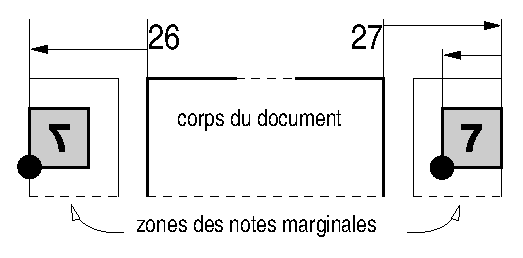
\includegraphics[width=.45\textwidth]{img/onglets}
\end{center}

因此,水平方向上的位置可以借助以下指令确定:

\begin{dmd}
\begin{verbatim}
\newcommand{\ongletIII}{%
    \makebox[0pt][l]{%
    \ifthenelse{\isodd{\value{page}}}{% 偶数页
        \hspace*{\marginparwidth}\hspace*{\marginparsep}%
        \hspace*{-\ongletwidth}\hspace{-2\fboxsep}}{% 奇数页
        \hspace*{-\marginparwidth}\hspace*{-\marginparsep}}%
        \b@iteonglet}}\end{verbatim}
\end{dmd}

这是因为,对于标签字盒的宽度来说,需要计入两次由指令\verb|\colorbox|确定的尺寸\verb|\fboxsep|。

\subsubsection{在竖直方向上确定位置}

剩下要做的就是去处理纵向位置的麻烦了……指令\verb|\raisebox|让我们可以在竖直方向上确定标签的位置。此外,借助以下格式,可以使\LaTeX 相信\codereplace{要移动的对象}的高度为零:

\begin{dmd}
\verb|\raisebox{|\codereplace{要移动的对象}\verb|}[0pt][0pt]{|\codereplace{要移动的对象}\}
\end{dmd}

这样一来,它周围的对象就不会带有错位,尤其是那些构成页眉的对象。例如,编写如下内容:

\begin{dmd}
\begin{verbatim}
\newcommand{\ongletIV}{% 
    \makebox[0pt][l]{% 
    \ifthenelse{\isodd{\value{page}}}{%
        \hspace*{\marginparwidth}\hspace*{\marginparsep}% 
        \hspace*{-\ongletwidth}\hspace{-2\fboxsep}}{% 
        \hspace*{-\marginparwidth}\hspace*{-\marginparsep}}% 
        \raisebox{2cm}[0pt][0pt]{\b@iteonglet}}}\end{verbatim}
\end{dmd}

由此,我们可以放置一个向上平移2厘米的标签:

\newcommand{\ongletIV}{% 
    \makebox[0pt][l]{% 
    \ifthenelse{\isodd{\value{page}}}{%
        \hspace*{\marginparwidth}\hspace*{\marginparsep}% 
        \hspace*{-\ongletwidth}\hspace{-2\fboxsep}}{% 
        \hspace*{-\marginparwidth}\hspace*{-\marginparsep}}% 
        \raisebox{2cm}[0pt][0pt]{\biteonglet}}}

\ifthenelse{\isodd{\value{page}}}{%
  \begin{flushright}
    \bfseries\thepage\ongletIV\\[-10pt]
    \rule{\textwidth}{.4pt}
  \end{flushright}}{%
  \begin{flushleft}
  \ongletIV\bfseries\thepage\\[-10pt]
    \rule{\textwidth}{.4pt}
  \end{flushleft}}

我们选用的用于定义字盒位置的方法如下。对于第$c$章:

\begin{itemize}
    \item 向下平移固定尺寸$d_f$。
    \item 在此基础上,叠加一个正比于$c$的平移,即第$c$章对应标签的平移量为
    
    \begin{center}
        $c\times$\codereplace{标签高度}$\times \alpha$
    \end{center}

    其中,$\alpha$是用于控制签标签间距的系数。如果$\alpha=1$,则相邻标签的位置严格相差字盒的高度;如果$\alpha=2$,则标签间会以字盒高度两倍为步长来分布,等等。
\end{itemize}

对于第一个平移:

\begin{dmd}
\begin{verbatim}
% 第一个标签的位置
\newlength{\ongletvshift}
\setlength{\ongletvshift}{2cm}\end{verbatim}
\end{dmd}

接下来,对于系数$\alpha$:

\begin{dmd}
\verb+\newcommand{\ongletsep}{1.37}+
\end{dmd}

我们声明一个用于确定标签位置的尺寸:

\begin{dmd}
\verb|\newlength{\ongletpos}|
\end{dmd}

现在,可以编写指令\verb|\onglet|了:

\begin{dmd}
\begin{verbatim}
\newcommand{\onglet}{% 
    \makebox[0pt][l]{%
        \ifthenelse{\isodd{\value{page}}}{% 
            \hspace*{\marginparwidth}\hspace*{\marginparsep}% 
            \hspace*{-\ongletwidth}\hspace*{-2\fboxsep}%
        }{% 
            \hspace*{-\marginparwidth}\hspace*{-\marginparsep}}%
        % 计算纵向位置
        \setlength{\ongletvpos}{%
            -\ongletvshift
            -\ongletheight*\real{\thechapter}*\real{\ongletsep}}% 
        % 确定标签位置 
        \raisebox{\ongletvpos}[0pt][0pt]{\b@iteonglet}}}\end{verbatim}
\end{dmd}

呼!它正常工作了……对于不属于附录的章节来说,是这样的。但对于附录中编号为A、B、C等的章节,它还是不太行。这是因为我们不能通过这样的编号来计算纵向位置。稍微看过\dm{book.cls}后,我们可以确定有这样的内容:

\begin{dmd}
\begin{verbatim}
\newcommand\appendix{\par 
\setcounter{chapter}{0}% 
\setcounter{section}{0}%
[...] 
\gdef\thechapter{\@Alph\c@chapter}}\end{verbatim}
\end{dmd}

这里,我们可以理解,当我们使用\verb|\appendix|开启附录部分时,章节的计数器会自动归零,并且生成大写字母。因此,需要找到一种应付方式,来让标签在我们来到附录后依然可以继续平移。我采用的解决方案比较简单,就是使用新的计数器来为章节和附录计数。为了达到这个目的,我们做如下声明:

\begin{dmd}
\verb|\newcounter{chapitre}|
\end{dmd}

我们可以立刻进一步说明想使用阿拉伯数字来生成编号:

\begin{dmd}
\verb|\renewcommand{\thechapitre}{\arabic{chapitre}}|
\end{dmd}

我们在\verb+\frontmatter+的定义中来为该计数器归零:

\begin{dmd}
\begin{verbatim}
\renewcommand\frontmatter{% 
    \cleardoublepage 
    \setcounter{chapitre}{1} 
    [...]
    }\end{verbatim}
\end{dmd}

接下来,每次调用指令\verb|\chapter|时,该计数器递增:

\begin{dmd}
\begin{verbatim}
\renewcommand{\chapter}{% 
\cleardoublepage 
\stepcounter{chapitre} 
\thispagestyle{plain} 
[...]
}\end{verbatim}
\end{dmd}

\section{\LaTeX 示例}

\begin{codelist}[11.31]{
    作为本章的结尾,我们介绍一下环境
    \dm{ltxexemple}。它可以用于
    在文档中展示\LaTeX 代码示例和相
    关结果……
}
\begin{verbatim}
作为本章的结尾,我们介绍一下环境
\ltxenv{ltxexemple}。它可以用于
在文档中展示\LaTeX{}代码示例和相
关结果……\end{verbatim}
\end{codelist}

\subsection{必要工具}

包\textsf{fancyvrb}提供了两个针对文件的功能。首先,指令\verb|\VerbatimInput|可以用于插入一个文件的内容。例如:

\begin{dmd}
\verb|\VerbatimInput[lastline=4]{corps/jouets.tex}|
\end{dmd}

该指令可以插入(\dm{jouets.tex}正是本章的源代码文件)\yz{
    此处展示的为原书部分代码。
}:

\begin{dmd}
\begin{verbatim}
\chapter{De nouveaux jouets}
\label{chap-jouets}

\begin{epigraphe}{Le Cantique des cantiques Ct \textbf{7} 11}\end{verbatim}
\end{dmd}

其次,环境\verb|VerbatimOut|可以做相反的工作:

\begin{dmd}
\verb|\begin{VerbatimOut}{|\codereplace{文件}\}\\
\verb|    |\codereplace{\LaTeX 代码}\\
\verb|\end{VerbatimOut}|
\end{dmd}

这样可以将\codereplace{\LaTeX 代码}存入名为\codereplace{文件}的文件。

第二个必要的工具的灵感来自文件\dm{latex.ltx}中指令\verb|\settowidth|、\verb|\settoheight|等的定义。这个指令可以获取对象总高度,也就是计算高度和深度的和:

\begin{dmd}
\begin{verbatim}
\newcommand{\hauteurtotale}[2]{% 
    % 存储要测量的对象
    \setbox\@tempboxa\hbox{{#2}}%
    % 获取高度
    \setlength{#1}{\ht\@tempboxa}% 
    % 在高度基础上加上深度
    \addtolength{#1}{\dp\@tempboxa}%
    % 排空临时字盒
    \setbox\@tempboxa\box\voidb@x}%\end{verbatim}
\end{dmd}

注意,这里使用了\TeX 的指令,\verb|\ht|和\verb|\dp|可以分别返回字盒的高度和深度,指令\verb|\setbox|等价于\TeX 的\verb|\savebox|,字盒\verb|\@tempboxa|是\LaTeX 使用的临时字盒。最后,字盒\verb|\voidb@x|是空字盒。

\subsection{环境\texttt{ltxexemple}的原则}

本章开头介绍的环境\dm{ltxexemple}比目前我们遇到的环境稍微复杂些。实际上,当我们写下如下指令的时候,一方面需要能够生成正如\codereplace{内容}的内容(也就是完全照抄),另一方面需要能够解释它,也就是像\LaTeX 的行为那样去处理它:

\begin{dmd}
\verb|\begin{ltxexemple}|\codereplace{内容}\verb|\end{ltxexemple}|
\end{dmd}

最终,我们就会知道,需要让\LaTeX 处理\codereplace{内容}\emph{两遍},而这是很难实现的。详细说来,一种规避这种问题的方案是将\codereplace{内容}存储在一个可以重复使用的文件中。这里的重复使用,要么是指照抄,要么是指由\LaTeX 去解释。如此一来,浮现出的第一个难点是储存内容的环境的创建:

\begin{dmd}
\begin{verbatim}
\newenvironment{ltxexemple}{% 
    \VerbatimEnvironment 
    \begin{VerbatimOut}{\jobname.exa}}{% begin条目
    \end{VerbatimOut}}% end条目\end{verbatim}
\end{dmd}

\begin{qquestion}
不要看到包的文档中没有记录就来问我指令\verb|\VerbatimEnvironment|是干什么用的,上面定义的环境有了它才能正常实现功能。
\end{qquestion}

我们写得很好看,但这个环境目前只能把其内容存储到文件中。因此,需要在环境的end条目中编写如下内容:

\begin{dmd}
\begin{verbatim}\end{verbatimOut}%
\VerbatimInput{\jobname.exa}% 照抄内容 
\input{\jobname.exa}% 由LaTeX解释内容\end{verbatim}
\end{dmd}

这样一来,

\newenvironment{ltxexemplei}{%
    \VerbatimEnvironment%
    \begin{VerbatimOut}[gobble=2]{\jobname.exa}}
    {%
    \end{VerbatimOut}%
    \VerbatimInput{\jobname.exa}%
    \input{\jobname.exa}}

% \newsavebox{\bitebxedminipage}

\newenvironment{boxedminipage}[2][c]{%
    \begin{lrbox}{\bitebxedminipage}%
    \begin{minipage}[#1]{#2}}{%
    \end{minipage}\end{lrbox}%
    \fbox{\usebox{\bitebxedminipage}}}

\begin{flushleft}
    \begin{boxedminipage}{.33\linewidth}
  \begin{dmd}
\begin{verbatim}
\begin{ltxexemplei}
    \LaTeX{}代码……
\end{ltxexemplei}\end{verbatim}
  \end{dmd}
    \end{boxedminipage}%
    \hfill 的结果是:\hfill
    \begin{boxedminipage}{.4\linewidth}
\begin{ltxexemplei}
    \LaTeX{}代码……
\end{ltxexemplei}
  \end{boxedminipage}
  \end{flushleft}

接下来要做的就是为这两个部分排版。这正是接下来我们的目的。

\subsection{装入字盒}

我们的思路是将内容装入两个字盒:

\begin{dmd}
\begin{verbatim}
\newsavebox{\b@iteentree}
\newsavebox{\b@itesortie}\end{verbatim}
\end{dmd}

这样做的目的是存储“入口”(entrée;代码)和“出口”(sortie;由\LaTeX 解释的代码)。因此,在end条文中,我们可以编写如下环境:

\begin{dmd}
\begin{verbatim}
[...]\end{verbatimOut}%
\begin{ltxexempleenv}% 拓宽边栏
    \savebox{\b@iteentree}{% 保存照抄代码
        \begin{minipage}{.57\linewidth}
            \VerbatimInput{\jobname.exa}
        \end{minipage}}%
    \savebox{\b@itesortie}{% 被解释的代码
        \begin{minipage}{.40\linewidth} 
            \setlength{\parindent}{10pt}% 默认为0pt
            \input{\jobname.exa}
        \end{minipage}}%
    \usebox{\b@iteentree}
    \usebox{\b@itesortie}
\end{ltxexempleenv}\end{verbatim}
\end{dmd}

环境\dm{ltxexempleenv}和我们讲到拓宽边栏\celan{\S 11.1.4}时介绍的很像,唯一的区别时这里切换到了\verb|\small|\yz{
    似乎没有?
}%TODO 是吗
,并对竖直方向的空白做出了一些调整。可以注意到,“入口”字盒占页面宽度的57\%,而“出口”字盒占40\%。这样一来,以下代码:

\begin{dmd}
\begin{verbatim}
\begin{ltxexempleii}
  \LaTeX{}代码……
  \par\noindent
  后面没了。
\end{ltxexempleii}\end{verbatim}
\end{dmd}

的效果是:

\makeatletter%



\newenvironment{ltxexempleii}{%
  \setlength{\fboxsep}{.5pt}%
  \VerbatimEnvironment%
  \begin{VerbatimOut}[gobble=2]{\jobname.exa}}{%
  \end{VerbatimOut}%
  \begin{ltxexempleenv}% ø\ccomment{pour agrandir les marges}ø
    \savebox{\b@iteentree}{% ø\ccomment{le code en verbatim}ø
      \begin{boxedminipage}{\ltxexinputwidthratio\linewidth}
        \VerbatimInput{\jobname.exa}
      \end{boxedminipage}}%
    \savebox{\b@itesortie}{%ø\ccomment{le code interprété}ø
      \begin{boxedminipage}{\ltxexoutputwidthratio\linewidth} 
        \setlength{\parindent}{10pt}% ø\ccomment{par défaut \texttt{0pt}}ø
        \input{\jobname.exa}
      \end{boxedminipage}}%
    \usebox{\b@iteentree}%
    \usebox{\b@itesortie}
  \end{ltxexempleenv}}%
\makeatother%

\begin{ltxexempleii}
  \LaTeX{}代码……
  \par\noindent
  后面没了。
\end{ltxexempleii}

在这里,我们展示了“入口”和“出口”字盒的边界,从而说明它们的尺寸。同样可以注意到,这里环境的begin条文实际是这样定义的:

\begin{dmd}
\begin{verbatim}
\pagebreak[3]% 我们建议于此处换页
\VerbatimEnvironment% 
\begin{VerbatimOut}[gobble=2]{\jobname.exa}\end{verbatim}
\end{dmd}

选项\dm{[gobble=2]}用于系统性地“吞掉”各行开头的两个字符,因为所有优秀的编辑器\jz{
    我当然指的是\makebox[0pt][l]{//}vi,不好意思,\textsf{Emacs}……
}都会为源文件各行首加上两个空格作为缩进。因此,如下代码:

\begin{dmd}
\begin{verbatim}
\begin{ltxexempleii}
\LaTeX{}代码……
\par\noindent
后面没了。
\end{ltxexempleii}\end{verbatim}
\end{dmd}

的效果是:

\begin{ltxexempleii}
\LaTeX{}代码……
\par\noindent
后面没了。
\end{ltxexempleii}

接下来有关排版的工作就是创建中间的竖条。这正是11.8.5小节的目标。在此之前,我们在为示例编号这件工作上的进度延迟了些。

\subsection{示例的编号}

为了给示例编号,我们需要声明一个计数器\celan{\S 4.1}:

\begin{dmd}
\verb|\newcounter{c@exemple}[chapter]|
\end{dmd}

这个计数器应该在各章首归零。在将其作为引用之时,我们需要详细指明它的呈现方式:

\begin{dmd}
\begin{verbatim}
\renewcommand{\thec@exemple}{% 
    \thechapter.\arabic{c@exemple}}\end{verbatim}
\end{dmd}

每次调用环境\dm{ltxexemple}时,我们都调用如下指令:

\begin{dmd}
\verb|\refstepcounter{c@exemple}|
\end{dmd}

该指令可以使计数器递增,并为系统的引用更新改值。你在示例中间看到的小黑字盒宽度为\verb|\l@rgeurnumex|(定义为16 pt),由如下代码生成:

\begin{dmd}
\begin{tabbing}
1234567890123456789012345678901234567890\= \kill
\verb|\newcommand{\affichenumex}{% |\\
\verb|    \raisebox{-1.7pt}[0pt][0pt]{% |\\
\verb|        \setlength{\fboxsep}{.7pt}% |\\
\verb|        \colorbox{black}{%|\> $\leftarrow$\textsf{黑色字盒}\\
\verb|            \makebox[\l@rgeurnumex]{%|\> $\leftarrow$\textsf{宽度固定的字盒}\\
\verb|                \color{white}%|\> $\leftarrow$\textsf{内容展现为白色}\\
\verb|                \tiny\textsf{\thec@exemple}}}}}|
\end{tabbing}
\end{dmd}

这样一来:

\newcounter{cexemple}[chapter]
\renewcommand{\thecexemple}{% 
\thechapter.\arabic{cexemple}}
\setcounter{cexemple}{34}

\newcommand{\affichenumex}{% 
\raisebox{-1.7pt}[0pt][0pt]{% 
\setlength{\fboxsep}{.7pt}%
\colorbox{black}{% 
\makebox[16pt]{%
\color{white}%
\tiny\textsf{\thecexemple}}}}}

\begin{codelist}[11.34]{
小字盒(\affichenumex)
}
\begin{verbatim}
小字盒(\affichenumex)\end{verbatim}
\end{codelist}

因此,环境\verb|ltxexemple|可以更新为如下版本:

\begin{dmd}
\begin{verbatim}
\newenvironment{ltxexempleiii}{%
\VerbatimEnvironment%
\begin{VerbatimOut}[gobble=2]{\jobname.exa}}{%\end{verbatimOut}%
\begin{ltxexempleenv}% \end{verbatim}
\verb+    \refstepcounter{c@exemple}% +\quad$\leftarrow$\textsf{计数器递增}
\begin{verbatim}
    \savebox{\b@iteentree}{ [...] }% 
    \savebox{\b@itesortie}{ [...] }%
    \usebox{\b@iteentree}%
    \kern2pt%
    \parbox{3pt}{\rotatebox{90}{\affichenumex}}%
    \kern2pt%
    \usebox{\b@itesortie}
\end{ltxexempleenv}}%\end{verbatim}
\end{dmd}

效果如下:

\makeatletter
\newenvironment{ltxexempleiii}{%
  \setlength{\fboxsep}{.5pt}%
  \VerbatimEnvironment%
  \begin{VerbatimOut}[gobble=2]{\jobname.exa}}{%
  \end{VerbatimOut}%
  \begin{ltxexempleenv}% ø\ccomment{pour agrandir les marges}ø
    \refstepcounter{cexemple}
    \savebox{\b@iteentree}{% ø\ccomment{le code en verbatim}ø
      \begin{boxedminipage}{\ltxexinputwidthratio\linewidth}
        \VerbatimInput{\jobname.exa}
      \end{boxedminipage}}%
    \savebox{\b@itesortie}{%ø\ccomment{le code interprété}ø
      \begin{boxedminipage}{\ltxexoutputwidthratio\linewidth} 
        \setlength{\parindent}{10pt}% ø\ccomment{par défaut \texttt{0pt}}ø
        \input{\jobname.exa}
      \end{boxedminipage}}%
    \usebox{\b@iteentree}%
    \kern2pt%
    \parbox{3pt}{\rotatebox{90}{\affichenumex}}%
    \kern2pt%
    \usebox{\b@itesortie}
  \end{ltxexempleenv}}%
\makeatother%

\begin{ltxexempleiii}
  \setlength{\fboxsep}{-2pt}
  \setlength{\fboxrule}{.5mm}
  这个\fbox{例子}有点蠢……
\end{ltxexempleiii}

最后一个难点是处理引用系统。实际上,我们不能像这样编写:

\begin{dmd}
\verb|以下一个示例。\label{monexemple}|
\end{dmd}

这是因为,字符串\verb|\label{monexemple}|会出现在示例中:

\begin{codelist}[11.36]{
以下一个示例。
}
\begin{verbatim}
以下一个示例。\label{monexemple}\end{verbatim}
\end{codelist}

我们不希望这样……对此,这里采用的解决方案是,以一个指令作为媒介,将可能出现的标签\verb|\label|传递给环境。编写如下代码:

\begin{dmd}
\begin{verbatim}
\newcommand{\l@belex}{} % 当前标签值
% 用于更新标签的指令 
\newcommand{\labelexemple}[1]{%
\renewcommand{\l@belex}{#1}}\end{verbatim}
\end{dmd}

这样一来,在使用环境\dm{ltxexemple}前,只需要调用如下指令:

\begin{dmd}
\verb|\labelexemple{|\codereplace{标签}\}
\end{dmd}

这样,就可以在接下来的过程中使用\verb|\ref{|\codereplace{标签}\verb+}+或等价指令来引用它。在环境\dm{ltxexemple}的定义中,新增如下内容:

\begin{dmd}
\begin{verbatim}
% 如果当前标签不为空
\ifthenelse{\equal{\l@belex}{}}{}{%
    \label{\l@belex}}% 放置一个标签\end{verbatim}
\end{dmd}

用法语来讲,这里的意思是:“如果指令\verb|\l@belex|被定义为非空的值,我们就使用这个值来放置标签(指令\verb|\label|)”。接下来,需要将指令\verb|\l@belex|设置为空值,因为有一些情况与此相反,会多次定义标签(\LaTeX 的消息“Label ``$\times\!\times\!\times$''\ multiply defined”)。因此,我们可以这样写:

\begin{dmd}
\begin{verbatim}
% 如果当前标签不为空 
\ifthenelse{\equal{\l@belex}{}}{}{%
    \label{\l@belex}% 放置标签
    \renewcommand{\l@belex}{}}\end{verbatim}
\end{dmd}

从语法角度来讲,这样编写是正确的,但是这里指令\verb|\renewcommand|的有效范围是局部的,它被限制为只能在检测\verb|\ifthenelse|的区域内生效。为了规避这个问题,我们可以使用\TeX 的结构:

\begin{dmd}
\verb|\global\def\l@belex{}|
\end{dmd}

该结构可以代替\verb|\renewcommand|,从而使用全局的工作范围来重新定义。

\subsection{竖线}

剩余的工作来到了绘制两个字盒间那条有点丑的线条这边。第一件要做的事情是分别去测量两个字盒的总高,并保留其中的较大值。以下代码可以实现这个目的:

\begin{dmd}
\begin{verbatim}
% 测量入口字盒
\hauteurtotale{\tempodim}{\usebox{\b@iteentree}}%
% 测量出口字盒
\hauteurtotale{\hauteurdutrait}{\usebox{\b@itesortie}}% 
% 取较大值
\ifthenelse{\hauteurdutrait>\tempodim}{%
    \setlength{\tempodim}{\hauteurdutrait}}{}\end{verbatim}
\end{dmd}

当然,需要提前声明尺寸\verb|\hauteurdutrait|和\verb|\tempodim|。在11.8.1小节中,我们可以看到有关指令\verb|\settotoalheight|的介绍。

这里在入口和出口字盒间要绘制的黑线的尺寸严格等于\verb|\hauteurtrait|减去\verb|\l@rgeurnumex|(带有示例编号字盒的宽度)。我们存储该尺寸:

\begin{dmd}
\begin{verbatim}
% 出去编号字盒的线高
\setlength{\hauteurdutrait}{\tempodim-\l@rgeurnumex}\end{verbatim}
\end{dmd}

经过作者大会无记名投票,决定线条长度的70\%绘制在编号上方,30\%绘制在编号下方。因此,中央的线条由如下的\verb|\parbox|生成:

\begin{dmd}
\begin{verbatim}
% 中央的线条
\parbox{3pt}{%
    \begin{center}
        % 上方70% 
        \rule{3pt}{.7\hauteurdutrait}\\\nointerlineskip% 
        \rotatebox{90}{\affichenumex}\\\nointerlineskip% 
        % 下方30% 
        \rule{3pt}{.3\hauteurdutrait}%
    \end{center}}\end{verbatim}
\end{dmd}

因此,指令\verb|\nointerlineskip|可以删除竖直方向上所有多余的空白,而这些空白可能是由指令\verb|\\|插入的。在关于微型目录的小节\celan{\S 10.7.4}中,我们给出了更多的细节。

\begin{codelist}[11.37]{
好了,这就是关于这个出色的环境
\dm{ltexexemple}的全部内容。
注意,尺寸\dm{3pt}也可以是
某个长度定义的对象……
}
\begin{verbatim}
好了,这就是关于这个出色的环境
\ltxenv{ltexexemple}的全部内容。
注意,尺寸\texttt{3pt}也可以是
某个长度定义的对象……\end{verbatim}
\end{codelist}